\documentclass[conference]{IEEEtran}
\IEEEoverridecommandlockouts
% The preceding line is only needed to identify funding in the first footnote. If that is unneeded, please comment it out.
\usepackage{cite}
\usepackage{amsmath,amssymb,amsfonts}
\usepackage{algorithmic}
\usepackage{graphicx}
\usepackage{textcomp}
\usepackage{subfigure}
\usepackage{float}
\def\BibTeX{{\rm B\kern-.05em{\sc i\kern-.025em b}\kern-.08em
    T\kern-.1667em\lower.7ex\hbox{E}\kern-.125emX}}
\begin{document}

\title{Decontamination of black virus in chordal ring using parallel strategy
\\
{\footnotesize \textsuperscript{}}
\thanks{Identify applicable funding agency here. If none, delete this.}
}

\author{\IEEEauthorblockN{1\textsuperscript{st} Given Name Surname}
\IEEEauthorblockA{\textit{dept. name of organization (of Aff.)} \\
\textit{name of organization (of Aff.)}\\
City, Country \\
email address}
\and
\IEEEauthorblockN{2\textsuperscript{nd} Given Name Surname}
\IEEEauthorblockA{\textit{dept. name of organization (of Aff.)} \\
\textit{name of organization (of Aff.)}\\
City, Country \\
email address}
\and
\IEEEauthorblockN{3\textsuperscript{rd} Given Name Surname}
\IEEEauthorblockA{\textit{dept. name of organization (of Aff.)} \\
\textit{name of organization (of Aff.)}\\
City, Country \\
email address}
}

\maketitle

\begin{abstract}
In this paper we consider the Black Virus Decontamination (BVD) problem in chordal ring using parallel strategy. The Black Virus (BV) is a harmful entity endowed with the ability to destroy any agent arriving at the site where it resides and then to move to all its neighbouring sites. The BVD problem is to employ a team of agents to locate and permanently eliminate the BV. Different from the sequential strategy (using two agents in the exploring phase) for BVD problem in chordal rings which is time-consuming, our strategy explores the chordal ring parallelly (using a group of agent in the exploring phase) which decreases the time dramatically with acceptable cost and this advantage is more obvious when the size of the chordal ring is larger. In order to let the agents which are moving to the new-formed BVs when the original BV is triggered stop, we propose $Three\,Jump\,Notifying\,Technique$ to ensure that no agent are destroyed once the BV is located. In order to compare with the sequential strategy in time fairly, we introduce Total Working Time(TWT) which is calculated by multiplying the number of agents and the total execution time. Another advantage of our strategy is that the casualties also decrease.\end{abstract}

\begin{IEEEkeywords}
Black Virus, Graph Exploration and Decontamination, Mobile Agent.
\end{IEEEkeywords}

\section{Introduction}
Mobile agents are widely used in distributed and network systems while the applications of them can cause some security issues,thus threatening to the network: A contaminated or infected host can destroy working agents for various malicious purposes; A malicious agent can contaminate or infect other computer nodes so they become malfunctional or crash.The harmful hosts, often called $Black\,Holes$ trigger the problem called $Black\,Hole\,Search$, the focus of which is to locate their positions since they are static and this problem has been extensively studied (e.g.,          ). The harmful agents trigger the problem called $Intruder\,Capture$ (IC). Its main focus is to deploy a group of mobile agents to capture a extraneous mobile agent (the intruder) who moves arbitraily fast through the network and infects the visiting sites. Also this problem has been extensively investigated.
A new harmful presence called black virus BV has been initially introduced by Cai et al. in(               ). It is a dangerous process residing at an unknown site in a network and destroying any upcoming agents, but unlike the BH, the node where the original BV resides thus becomes clean. At the same time, the original BV multiplies (called clones) and spreads to all neighbouring nodes, thus increasing its number and damage in the network. A BV is destroyed when it moves to a site where there is already an agent. on this harmful presence, a new problem called Black Virus Decontamination(BVD) is presented by Cai et al., the main focus of which is to use a group of system agents to permanently remove any presence of the BV from the network. A protocol defining the actions of the agents solves the BVD problem if at least one agent survives and the network is free of BVs. Also, a desirable property of a decontamination protocol is that the nodes which have been explored or cleaned by mobile agents are not be recontaminated by the BV spreading. In \cite{Alotaibi}, solution for BVD in the chordal ring (sequential strategy) is discussed. In Alotaibi's thesis, she discuss solutions based on different kinds of chordal ring: double loops, triple loops, consecutive-chords rings and finally general chordal rings. \\
In this paper, we discuss parallel strategy on BVD problem in chordal ring. A chordal ring is a circulant graph with $d_1=1$, i.e., it is an augmented ring, and will be denoted by $C_n(1, d_2, ..., d_k)$. More specifically, in chordal ring each node is directly connected to the nodes at distance $d_i$ by additional links called chords. The link connecting two nodes is labeled by the distance that separate these two nodes on the ring. 
For convenience, if we say the agents or the clones move along chord $i$, then they actually move along $d_i$. If we say the agents or the clones move $i$, then they actually move along chord $d_x$ with its length equal to $i$. Let us donated by $d$ the half degree of the chordal ring (for example, for the chordal ring structure $C_n(1,2,4,5)$, $d=4$), by $l$ the length of the longest chord of the chordal ring (for example, for the chordal ring structure $C_n(1,2,4,5)$, $l=5$). In order to simplify the process, we assume that all the nodes in the network are marked with a number: the starting point is marked 0, then the second node is marked 1... Our goal is to minimize the time to complete the whole decontamination process and at the same time the casualties. In order to do that, we propose a parallel strategy for decontaminating the chordal ring. It is the first attempt to deal with this issue in a parallel way. Agents are not allowed to communicate with each other unless they are in the same node so the protocol should enable agents in different nodes to move properly. That is, the route of every agent is different but they are served to explore the network; when a BV is triggered, other agents should bypass the new-formed BVs. We give simple but efficient solution to deal with the problem with acceptable cost. 
In the elimination phase, we are interested in executing it also parallelly. But in this case, an tricky situation might happen: supposing that the sites of the two clones are connected, in this case, after these two clones are triggered, one of their clones spread to another sites and since the agents sent to destroy them die, these two sites are empty when the second round clones arrive, which make our decontamination invalid. In order to solve this problem, we make an assumption when we talk about the parallel strategy in elimination phase in chordal rings: when a BV is triggered at $T_i$, it takes negligible time for its clones to reach all its neighbours, for example, at $T_i$.  

\section{Shadowed Exploration}
\subsection{Initialization }
The chordal ring is a complete symmetrical structure, so we can randomly choose a node $x_0$ as the start node. Initially, we place $2d$ agents at node 0, 1, \ldots , $2d-1$ (first round). Agents residing in nodes from $0$ to $d-1$ are in shadowing group, while from $d$ to $2d-1$ are in exploring group. If none of the agent is destroyed, we then place $d$ agents at nodes 0,1, \ldots, $d-1$ (second round). If not, we can easily know the location of the BV and employ agents to surround the new formed BVs, then destroy them permanently. Only the agents employed in the first round move in the exploring phase. The agents employed in the second round remain dormant, guarding the nodes to guarantee the monotone. \\

\subsection{Route of the agent in exploring phase}
We separate the time of exploring phase into two part: moving time and notifying time. In the whole phase of exploring phase, they are arranged as below: $T_{move\_1}$, $T_{notify\_1}$, $T_{notify\_1'}$, $T_{notify\_1''}$, $T_{move\_2}$, $T_{notify\_2}$, $T_{notify\_2'}$, $T_{notify\_2''}$ \dots More specifically, every cycle contains one unit of time for moving and three units of time for notifying. We discuss why we arrange the time as above and what exactly the agents do in the notifying time later. 

In chord ring $C_n(1, d_2, \ldots, d_k)$, all the agents in the array move along their longest chord $d_k$ in $T_{move\_i}$. That is, agents move along $d_k$ in $T=1+4t$ $(t\in \mathbb{N})$.  An example of how agents move in chordal ring $C_n(1, 2 , 4, 5)$ at $T_{move\_i}$ in exploring phase is shown in Fig.\ref{fig:subfig1}. For our convenience, in some case, we consider the chordal ring as arranged in rows of $d_k$ where the last node of a row is connected to the first node of the following row and the last node is connected to the first. Depending on the size of the chordal, the last row could be incomplete. So in this matrix, moving down a column corresponding to using the longest chord $d_k$. In the matrix, we also mark the number of nodes.\\

\begin{figure}
  \centering 
  \subfigure[Arrangement of agents at $T_{move\_i}$]{ 
    \label{fig:subfig1:a} %% label for first subfigure 
    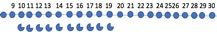
\includegraphics[width=3.0in]{figures/chordal_a_l.png}} 
  \hspace{1in} 
  \subfigure[Arrangement of agents at $T_{move\_{i+1}}$]{ 
    \label{fig:subfig1:b} %% label for second subfigure 
    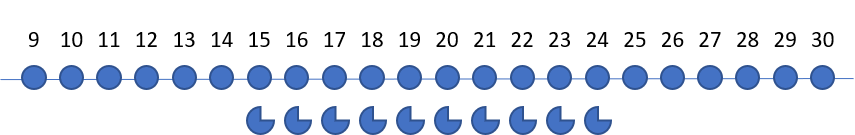
\includegraphics[width=3.0in]{figures/chordal_a1_l.png}}
  \caption{Arrangement of agents when moving} 
  \label{fig:subfig1} %% label for entire figure 
\end{figure}


\subsection{$Three\,Jump\,Notifying\,Technique$}
In the model of BV decontamination exploring the network sequentially, explore agent moves forward for one step. If the node is safe, it move back to the leader agent, and then move forward to the safe node together. In this case, if the leader agent does not meet the leader in next $T$ after it moves forward, the leader agent learns that the original BV resides in the next node so it stop moving. 
But in our model, we employ $2d$ agents in the exploring phase, if they are not properly informed when one agent is destroyed by BV, in their next step of moving, some of them may be destroyed by the new formed BVs. In order to avoid the casualties, we propose $Three\,Jump\,Notifying\,Technique$ to properly notify the agents who will move to the new formed BVs.
For convenience, let us take the node where the original BV resides as the original of the one-dimensional coordinate system. In a chordal ring $C_n(1, d_2, \ldots,  d_k)$, if the original BV is triggered, the clones of it spread to nodes whose coordinates are $-d_k$, $-d_{k-1}$, \ldots, $-d_2$, $-1$, $1$, $d_2$, \ldots, $d_{k-1}$, $d_k$. Obviously the nodes whose coordinates are $1$, $d_2$, \dots, $d_{k-1}$, $d_k$ may become the BV (Possible BV Nodes) now, our goal is to notify the agents which will move to these nodes to stop ($Risky\,Agent$). The coordinates of them are $1- d_k$, $d_2-d_k$, \ldots, $d_{k-1}-d_k$, $d_k-d_k$ (which is exactly the coordinate of the original BV) respectively. It is obvious that not all of the nodes from $1$ to $d_k$ become BV nodes after the triggering because there might be some agents already there, but since notifying all the $Risky\,Agents$($RA$s) does not add more cost comparing to notifying some of them, in our strategy, we notify all of the $RA$s. Let us donate one of the Possible BV Nodes by $d_i$, and in our $Three\,Jump\,Notifying\,Technique$, agent residing in node $-d_i$ ($Notification\,Agent$) is employed to notify the agent residing in node $-d_k+\left |d_i\right |$ (RA) who will move to the BV node. 

We show that $Notification\,Agent$ ($NA$) are able to meet RA in three steps: $-d_i\xrightarrow[]{move\left | d_i \right |}0\xrightarrow[]{move\,along\,chord\,k}-d_k\xrightarrow[]{move\,\left | d_i \right |}-d_k+\left|d_i\right|$. In this case, the notifying route of the $NA$ whose coordinate is $-d_k$ is $-d_k{\rightarrow}0{\rightarrow}-d_k{\rightarrow}0$ . We would make some modification in the $Surrounding\,and\,Elimination$, but now let us assume it still follow the route above. The whole process of $Three\,Jump\,Notifying\,Technique$ in chordal ring $C_n(1, 2, 4, 5)$ is shown in Fig.\ref{fig:subfig}. 

\begin{figure}
  \centering 
  \subfigure[Arrangement of agents at $T_{move_i}$]{ 
    \label{fig:subfig:a} %% label for first subfigure 
    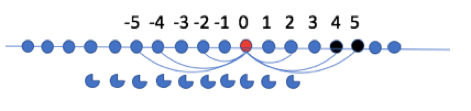
\includegraphics[width=2.5in]{figures/tjt1.png}} 
  \hspace{1in} 
  \subfigure[Arrangement of agents at $T_{notify_i}$]{ 
    \label{fig:subfig:b} %% label for second subfigure 
    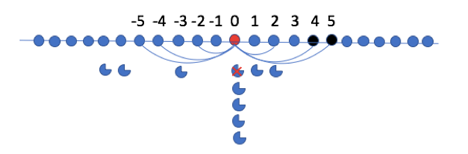
\includegraphics[width=2.5in]{figures/tjt2.png}} \
  \hspace{1in} 
  \subfigure[Arrangement of agents at $T_{notify_i'}$]{ 
    \label{fig:subfig:c} %% label for second subfigure 
    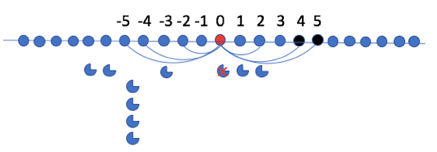
\includegraphics[width=2.5in]{figures/tjt3.png}} 
  \hspace{1in} 
  \subfigure[Arrangement of agents at $T_{notify_i''}$]{ 
    \label{fig:subfig:d} %% label for second subfigure 
    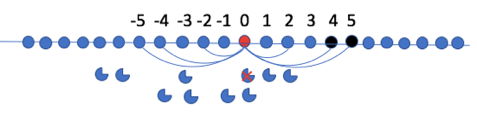
\includegraphics[width=2.5in]{figures/tjt4.png}} 
  \caption{The whole process of the $Three\,Jump\,Notifying\,Technique$ in chordal ring $C_n(1, 2, 4, 5)$} 
  \label{fig:subfig} %% label for entire figure 
\end{figure}


If the original BV residing in the red node, then once an agent moves to it, the agent and the BV are destroyed but the clones of the BV spread to all its neighbours. According to our technique, nodes whose coordinates are $1$, $2$, $4$, $5$ become $Possible\,BV\,Nodes$; agents residing in nodes $-4$, $-3$, $-1$, $0$ are the $RA$s; agents residing in nodes $-5$, $-4$, $-2$, $-1$ are the $NA$s. The routes for agents residing in nodes $-5$, $-4$, $-2$, $-1$ are $-5{\rightarrow}0{\rightarrow}-5{\rightarrow}0$; $-4{\rightarrow}0{\rightarrow}-5{\rightarrow}-1$; $-2{\rightarrow}0{\rightarrow}-5{\rightarrow}-3$; $-1{\rightarrow}0{\rightarrow}-5{\rightarrow}-4$ respectively.\\

\subsection{Safe Exploring with $Three\,Jump\,Notifying\,Technique$}

After the initialization, agents employed in the first round move as the route we introduced in ``Route of the agent in exploring phase'' . When one of the agents is destroyed at $T_{move_i}$, then $Three\,Jump\,Notifying\,Technique$ begins. In ``Route of the agent in exploring phase", we say that in the exploring phase every cycle contains one unit of time for moving and three units of time for notifying. Actually, the three units of time for notifying are reserved for $Three\,Jump\,Notifying\,Technique$, even though it only executes when one of the agents is destroyed. In another word, before encountering a BV, all the agents just stay where they are in the notifying time.
After executing the $Three\,Jump\,Notifying\,Technique$, the $NA$ moves back to where they are before the notification. For example, in the example in $Three\,Jump\,Notifying\,Technique$, $NA$ residing in node $-1$ moves back to node $-4$ following the reverse route in the notifying phase which is $-1{\rightarrow}-5{\rightarrow}0{\rightarrow}-4$. 

\section{Surrounding and Elimination}
It is obvious that not all the agents are informed to stop so we call the agents contining to move the $KeepMoving$ agents. In this section, we introduce the process of eliminating the BVs after the original BV is triggered. For the purpose of saving the number of agents, we prefer to chase the $Keep\,Moving$ agents, but it is not necessary to complete the process, for example, you can carry enough number of agents so you can proceed the $Surrounding\,and\,Elimination$ immediately. Here, we only focus on chasing the $KeepMoving$ agents.

\subsection{Notifying Moving Agents}

\noindent{\bf Overview of the Notifying Moving Agents}

When the $Shadowed\,Exploring$ ends, it is possible that some of the agents in the array are not informed and do not realize the existence of the BV, so they keep moving following the routes in $Shadowed\,Exploring$  phase but it is obvious that they would not encounter any BV. In order to reduce waste, we employ the agent who receives the clone from chord $d_k$ ($Coordinate\,Agent$) to notify the other $Keep\,Moving$ agents to move back to their position when the BV is triggered. Now we introduce how we choose the $Coordinate\,Agent$($CA$)and how the $CA$ notifies the other agents.\\

\noindent{\bf The Process of the Notifying Phase of the Coordination Agent}

We can see that the relative position of agents does not change when they keep moving along the longest chord. For example, agents residing in nodes 1, 5, 10 (noted as $A1$, $A5$, $A10$) move along the longest chord and then $A5$ moves forward for one step. The relative position of them would be exactly the same as the situation where all of them remain dormant except $A5$ moves forward for one step. Now we discuss how the $CA$ notify all the $Keep\,Moving$ agents assuming they are dormant and then make some modification to fit the scenario where the $CA$ notifies the $Keep\,Moving$ agents. The problem we need to solve is that given a range within which the agents are in and a $CA$ located in this range, let the $CA$ to notify all the agents in this range. In a chord ring $C_n(1, d_2, \ldots, d_k)$, the $CA$ sets a $Notification\,Window$ using the modular arithmetic. Let us assume the number of the node where the $CA$ resides in is $x$, the number of the nodes where should be marked the $Beginning\,Flag$ and the $End\,Flag$ are $y$ and $z$. 

The relations between $x$, $y$, $z$ should be as follow: 

\begin{itemize}
\item $y$ is the biggest number which satisfies that it is smaller than or equal to $x$ and that $y$ mod $d_k$ =$0$; 
\item $z$ is the smallest number which satisfies that it is bigger than $x$ and that $z$ mod $d_k$ = $d_{k-1}$.
\end{itemize} 


When the agent is chosen to be the $CA$, it computes its $Notification\,Window$. When we mention marking a flag, it does not mean that the agent has to move to the node to do that but only needs to remember the positions of the two flags in its memory. Also, after the position of the $Notification\,Window$ is set, it remains stable. More specifically, when the $CA$ moves, he does not set another $Notification\,Window$ using its new position. The $CA$ moves step by step to every possible position and notifies the agents to go back if there is one until it realizes that it just passes the $End\,Flag$. After that, he moves along the longest chord anticlockwise to the node marked a $Beginning\,Flag$ and continues moving again step by step to notify agents until it arrives its relative departing node. For example, if the $CA$ starts to notify other from node $x$, then its relative departing node is $x'=x+t\times{d_k}$ ($t\in \mathbb{N}$).

We make some modifications to let the solution fit the real scenario where the agents move along the longest chord: 
\begin{itemize}
\item The Beginning Flag and the End Flag move along the longest chord also to keep the relative position the same. 
\item  When one agent $A1$ moves to a node where there is an agent $A2$ knowing the position of the original BV, $A1$ would be informed and directly moves along the longest chord to its own position. 
\item  Let us assume that the time when the original BV is triggered is $T_{move\_i}$ ($T_{trigger}$), then the $CA$ should remember the $T_{trigger}$ and informs the agents he encounters of it. The agent $A1$ who encounters the $CA$ should remember the time when they encounter ($T_{notify\_now}$) and stop moving until next $T_{move}$ when it will meet another agent $A2$. Then $A1$ moves along $d_k$ anticlockwise for $T_{move\_now}-T_{trigger}$ times while $A2$ moves for $T_{move\_now}-T_{trigger}+1$ times. 
\item When arriving its relative departing position at $T_{move\_a}$, the $CA$ knows that it has finished the task and moves along $d_k$ for $T_{move\_a}- T_{trigger}+1$ times to its position when the original BV is triggered.
\item Let us assume that the time when the BV is triggered is $T_{move\_i}$, the $CA$ starts to move step by step to notify other agents after $T_{move\_{i+2}}$, because we want to ensure the security of the $CA$. If it starts to notify other agents at $T_{move\_{i+1}}$, it might encounter a BV. Also, it should be ensured that the $Keep\,Moving$ agents in the exploring group are in the $Notification\,Window$ of the $CA$, or the $CA$ would never encounter them. We would talk about how to ensure this in next section.
\end{itemize} 

\noindent{\bf Election of the Coordination Agent}

We choose the agent who receives a BV clone from its chord $d_k$ to be the $CA$, which means when an agent receives a BV clone from its longest chord, then it realizes that it is chosen as the $CA$. We know that, the notifying phase starts from $T_{move\_{i+2}}$ assuming the time when the BV is triggered is $T_{move\_i}$, which means the notifying phase begins only after all the $Keep\,Moving$ agents move twice. At $T_{move\_{i+2}}$, all the $Keep\,Moving$ agents are in a $Notification\,Window$ from nodes $d_k\times(move\_{i}+1)\,to\,d_k\times(move\_{i}+1) + d_{k}-1$, and let us donate it by $Initial\,Notification\,Window$. The $CA$ would directly move to any node in $Initial\,Notification\,Window$. Now we propose three kinds of routes for the $CA$ to move to his destination:

The coordinates of the positions where the clones spread are: $x-d_k$ (which is the coordinate of the $CA$), $x-d_{k-1}$, $x-d_{k-2}$, \ldots, $x-1$, $x+1$, $x+d_2$, \ldots, $x+d_{k-1}$, $x+d_{k}$ supposing the coordinate of the original BV is $x$ and we are in a chordal ring $C_n(1, d_2,\ldots, d_k)$.
 Now we describe three scenarios:
\begin{itemize}
\item Scenario 1: The last agent of the $Exploring\,Group$ is destroyed by the BV and the positions of the clones satisfy: $x-d_{k-1}+d_{k}=x+1$, $x-d_{k-2}+d_{k}=x+d_2$, \ldots, $x-1+d_{k}=x+d_{k-1}$. 
\item Scenario 2: The last agent of the $Exploring\,Group$ is destroyed by the BV and the at least one pair of the positions of the clones does not satisfy: $x-d_{k-1}+d_{k}=x+1$, $x-d_{k-2}+d_{k}=x+d_2$, \ldots, $x-1+d_{k}=x+d_{k-1}$. 
\item Scenario 3: One of the agents in the $Exploring\,Group$ except the last agent is destroyed by the BV.
\end{itemize}

In scenario 1, the $CA$ needs to move for 5 steps to reach its destination while in the other two scenarios, it only needs to move for 4 steps to arrive the destination. Now we propose the route for each scenario.
\begin{itemize}
\item For $CA$ in scenario 1: Let us donate by $y$ the coordinate of the node in the $Notification\,Window$ set by the original BV which does not receive any clone and his left neighbour receives a clone (the coordinate of it is $y-1$). The $CA$ first moves to the original BV, then to node $y-1$, finally to $y$. After that it only need to move along the chord $d_k$ for twice to reach its destination.
\item For $CA$ in scenario 2: There is at least one pair of the positions of the clones does not satisfy the equations so there should be one node (assuming its coordinate is $z$) who receives a clone from the original BV but node $z+d_k$ is empty. The route now for the $CA$ is first move to the BV, then to node $z$, and then moves along the chord $d_k$ for twice to reach its destination.
\item For $CA$ in scenario 3: The $CA$ here simply need to move for one step to its right neighbour and move along the chord $d_k$ for three times to reach its destination.
\end{itemize}


In any case, the $CA$ can reach its destination within 6 unit of time which is required for the $Keep\,Moving$ agents to move to the $Initial\,Notification\,Window$, so the $CA$ start to chase the $Keep\,Moving$ agents as we introduce from $T_{notify\_{i+2}}$. 

An example of how the agents and the $CA$ move in chordal ring $C_n(1, 2, 7, 11)$is shown in \ref{fig:T29}. 
\begin{figure}[H]
  \centering  
  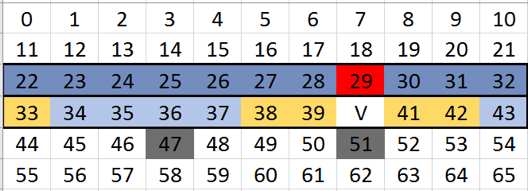
\includegraphics[width=0.4\textwidth]{figures/T29.png}
  \caption{Arrangement of agent at $T_{move\_2}$ when the BV is triggered}\label{fig:T29}
\end{figure}

Yellow nodes are connected to the original BV but guarded by agents while the grey nodes are the new formed BVs. The node marked $V$ is the original BV but now is clean. Agent residing in node 29 receives clone from chord $d_k$ so it knows it is the $CA$ During the notifying time, agents residing in nodes 33, 38, 39 notify agents residing in nodes 36, 31, 30 respectively following the $Three\,Jump\,Notifying\,Technique$ while the $CA$ moves to 28, 39, 50 and finally 61 following the route in scenario 3.

\begin{figure}[H]
  \centering  
  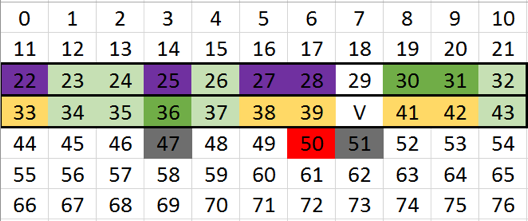
\includegraphics[width=0.4\textwidth]{figures/T50.png}
  \caption{Agents roles after $Three\,Jump\,Notifying\,Technique$ and choosing $CA$. (for convenience, we donate the $CA$ by a red spot, more specifically, node 50 is where $CA$ resides)}\label{fig:T50}
\end{figure}

Agents in purple nodes would be notified at $T_{move\_3}$ and move back. Agents in light green nodes are the $Keep\,Moving$ agents while agent in dark green nodes are informed to stop in $Three\,Jump\,Notifying\,Technique$. In the meantime, the $CA$ moves to node 28, 39, 50, and finally 61. It is obvious that the $CA$ can reach its destination before $T_{move_4}$, so it waits until $T_{notify_4}$ to start its notifying phase. 

\begin{figure}[H]
  \centering  
  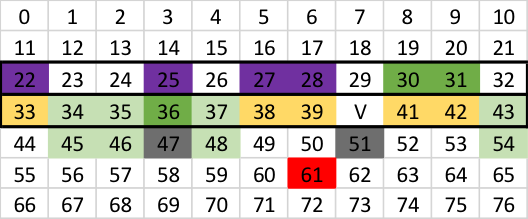
\includegraphics[width=0.4\textwidth]{figures/T611.png}
  \caption{Arrangement of agent at $T_{move\_3}$. The $CA$ has arrived its destination)}\label{fig:T611}
\end{figure}

\begin{figure}[H]
  \centering  
  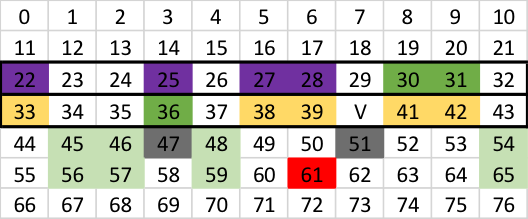
\includegraphics[width=0.4\textwidth]{figures/T612.png}
  \caption{Arrangement of agents at $T_{move_4}$. The $CA$ starts its notifying phase}\label{fig:T612}
\end{figure}
In notifying phase, $CA$ starts to notify other $Keep\,Moving$ agents. First, it computes the $Notification\,Window$ which is from node 55 to node 65. Note that the $Notification\,Window$ would move along chord $d_k$ at every $T_{move}$. It moves to node 62 at $T_{notify\_4}$, node 63 at $T_{notify\_4'}$, node 64 at $T_{notify\_4''}$ and to node 75 at $T_{move\_5}$.

\begin{figure}[H]
  \centering  
  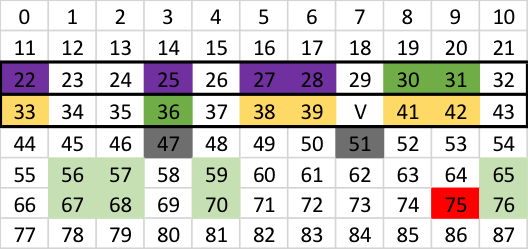
\includegraphics[width=0.4\textwidth]{figures/T75.png}
  \caption{Arrangement of agents at $T_{move_5}$. }\label{fig:T75}
\end{figure}
Again, in the notifying phase, $CA$ moves to node 76 at $T_{notify\_5}$. We can see that it encounters agent residing in node 76, so $CA$ informed it the $T_{trigger}$ which is $T_{move\_2}$. Agent residing in node 76 should remember $T_{notify\_now}$ which is $T_{notify\_5}$ and wait until next $T_{move}$ to inform agent ($Following\,Agent$) who resides in node 65 now but would move to node 76 next $T_{move}$. After encountering its $Following\,Agent$, it informs it to move back along chord $d_k$ for $T_{move\_now}-T_{trigger} +1$ times which is $T_{move\_5}- T_{move\_2}+1$ times while itself moves for $T_{move\_5}$- $T_{move\_2}$ times. 
At $T_{T_{notify\_5'}}$ when the $CA$ arrives at node 77, it knows that it just pass its $Ending\,Flag$ so it moves along the longest chord anticlockwise to its $Beginning\,Flag$ at $T_{notify\_5''}$.
\begin{figure}[H]
  \centering  
  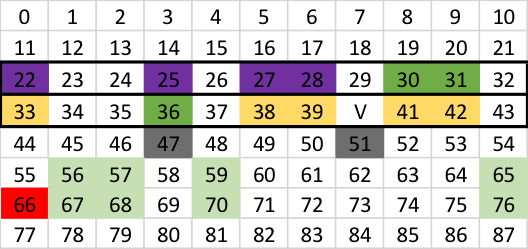
\includegraphics[width=0.4\textwidth]{figures/T66.png}
  \caption{Arrangement of agents at $T_{move_5''}$. }\label{fig:T66}
\end{figure}

\begin{figure}[H]
  \centering  
  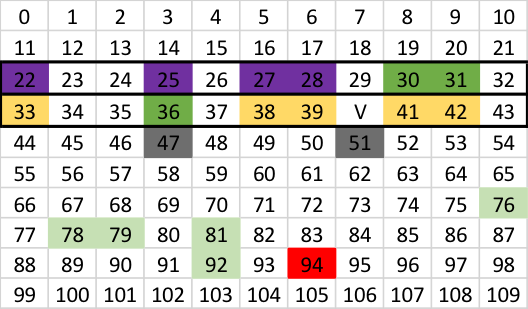
\includegraphics[width=0.4\textwidth]{figures/T94.png}
  \caption{Arrangement of agents at $T_{move_7''}$. }\label{fig:T94}
\end{figure}

We could know that the $CA$ moves back to its relative original position at $T_{notify\_7''}$. It would wait until next $T_{move}$ to inform its $Following\,Agent$ of $T_{trigger}$ and moves back with it.

\subsection{Overview of the Elimination}
After all the agents move back to where they are when the BV is triggered, we start the $Surrounding\,and\,Elimination$. We are interested in destroying the BVs at one time. So we need to first guard all the neighbouring nodes of the new formed BVs. In order to avoid collision and efficiently leverage the agents, we allocate different Destination Tables to all the agents in the array to inform them where should they should move in different situations (e.g., when the first agent in the exploring team is destroyed, then every agent except the first agent have a distinct destination, when the second agent is destroyed, then every agent except that agent destroyed have a distinct destination. More specifically, for a Chord Ring with half degree $d$, every agent in the array carries a $Destination\,Table$ with $d-1$ destinations. If we need more agents, then we will give their $Destination\,Table$ to the last agent in the shadowing group, when the elimination begins, it clones enough number of agents and give the $Destination\, Table$ to them. Before moving to its destination, the agent computes the shortest route from its own position to its destination using Dijkstra Algorithm. There are two kinds of agent in the Elimination phase: surrounding agents who are responsible for guarding the neighbouring nodes of the BVs and destroying agents who move to the BVs after all the neighbouring nodes are guarded. We want the BVs to be destroyed at one time, so it is important that the destroying agents move to the BVs at the same time and only after all the neighboring nodes are guarded by agents. In fact, if the destroying agents know the longest time $t_{longest}$ to move to the destination taken by all the agents (including the destroying agents and the surrounding agents), then they move to the last node prior to the destination and wait until $t_{longest}$ to move to the BVs together. So in the $Destination\,Tables$ for the destroying agents, we also add an item which is the $t_{longest}$. Now we introduce how to compute the shortest routes and how we design the $Destination\,Tables$. Note that we design $Destination\,Tables$ for all the agents and allocate them to the agents before the exploring phase begins.

\subsection{Destination Table and Elimination}
Supposing there are some BVs and agents in the chordal ring, it is obvious that the BV nodes are in the clockwise side of the agents. In order to use Dijkstra, first we need to map the chordal ring with BVs into a graph. We include nodes from the node containing the first agent to the node which is $d_k$ away from the last BV node, then delete the chords from the BV nodes to build the graph where we run Dijkstra Algorithm.
Here is an example how we built the graph for running Dijkstra Algorithm. Below we show the situation when the third agent in the exploring group is destroyed by the BV (see \ref{fig:D1}). Only the chords of the original BV node are shown. 
\begin{figure}[H]
  \centering  
  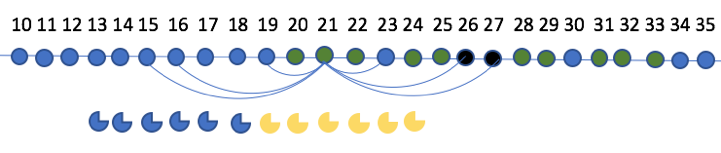
\includegraphics[width=0.4\textwidth]{figures/D1.png}
  \caption{Situation when the third agent in the exploring group is destroyed}\label{fig:D1}
\end{figure} 

The black node is the BV node while the green nodes need to be guarded. So in this case, we need 12 agents (10 surrounding agents and 2 destroying agents). 
We add nodes from 13 to 33 with their chords within this area and delete chords connected with the BV nodes to get the graph where we use Dijkstra Algorithm. Below is the graph we build. (see \ref{fig:D2}) For convenience, we show the all the nodes we included and the chords we delete.
\begin{figure}[H]
  \centering  
  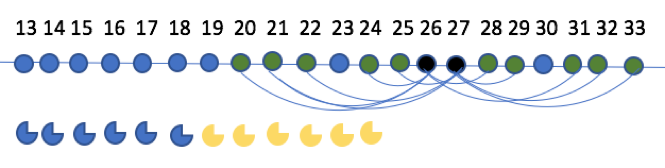
\includegraphics[width=0.4\textwidth]{figures/D2.png}
  \caption{The graph we build for Dijkstra Algorithm}\label{fig:D2}
\end{figure} 
Using the graph and Dijkstra Algorithm, we compute the routes from every agent to every node. Then we use enumeration to choose an allocation of every agents's destination satisfying: 
\begin{itemize}
\item 1) the maximum length of the route should be minimum. 
\item 2) after the allocation, in every needed position there should be exactly one agent.
\end{itemize}
After we get the optimal allocation, we record every agent?s distinct destination and the position of the third agent in the exploring group in their $Destination\,Table$. Also, we add the length of the longest chord to every destroying agent.
More specifically, here we talk about the situation when the third agent in the exploring group is destroyed. For every agent, the information we compute would be in the third part of its $Destination\,Table$ recording the position of the third exploring agent (for example, it connects this agent through chord $x$), the destination it should move if the third exploring is destroyed. For a destroying agent, there should be another item recording the length of the longest route in this part.
Above we introduce how to design one part of $Destination\,Table$ of an agent, for every agent in chordal ring, it should hold a $Destination\,Table$ of $d-1$ parts, and every part contains 2 items (for surrounding agent) or 3 items (for destroying agent).
After the one of the agent is destroyed, the agent can check their $Destination\,Table$ to get the information of their destination. Then using Dijkstra Algorithm they can compute the shortest route separately and starts to move.


\section*{Acknowledgment}

The preferred spelling of the word ``acknowledgment'' in America is without 
an ``e'' after the ``g''. Avoid the stilted expression ``one of us (R. B. 
G.) thanks $\ldots$''. Instead, try ``R. B. G. thanks$\ldots$''. Put sponsor 
acknowledgments in the unnumbered footnote on the first page.

\section*{References}

Please number citations consecutively within brackets \cite{b1}. The 
sentence punctuation follows the bracket \cite{b2}. Refer simply to the reference 
number, as in \cite{b3}---do not use ``Ref. \cite{b3}'' or ``reference \cite{b3}'' except at 
the beginning of a sentence: ``Reference \cite{b3} was the first $\ldots$''

Number footnotes separately in superscripts. Place the actual footnote at 
the bottom of the column in which it was cited. Do not put footnotes in the 
abstract or reference list. Use letters for table footnotes.

Unless there are six authors or more give all authors' names; do not use 
``et al.''. Papers that have not been published, even if they have been 
submitted for publication, should be cited as ``unpublished'' \cite{b4}. Papers 
that have been accepted for publication should be cited as ``in press'' \cite{b5}. 
Capitalize only the first word in a paper title, except for proper nouns and 
element symbols.

For papers published in translation journals, please give the English 
citation first, followed by the original foreign-language citation \cite{b6}.

\begin{thebibliography}{00}
\bibitem{b1} G. Eason, B. Noble, and I. N. Sneddon, ``On certain integrals of Lipschitz-Hankel type involving products of Bessel functions,'' Phil. Trans. Roy. Soc. London, vol. A247, pp. 529--551, April 1955.
\bibitem{b2} J. Clerk Maxwell, A Treatise on Electricity and Magnetism, 3rd ed., vol. 2. Oxford: Clarendon, 1892, pp.68--73.
\bibitem{b3} I. S. Jacobs and C. P. Bean, ``Fine particles, thin films and exchange anisotropy,'' in Magnetism, vol. III, G. T. Rado and H. Suhl, Eds. New York: Academic, 1963, pp. 271--350.
\bibitem{b4} K. Elissa, ``Title of paper if known,'' unpublished.
\bibitem{b5} R. Nicole, ``Title of paper with only first word capitalized,'' J. Name Stand. Abbrev., in press.
\bibitem{b6} Y. Yorozu, M. Hirano, K. Oka, and Y. Tagawa, ``Electron spectroscopy studies on magneto-optical media and plastic substrate interface,'' IEEE Transl. J. Magn. Japan, vol. 2, pp. 740--741, August 1987 [Digests 9th Annual Conf. Magnetics Japan, p. 301, 1982].
\bibitem{b7} M. Young, The Technical Writer's Handbook. Mill Valley, CA: University Science, 1989.
\end{thebibliography}

\end{document}
